% T1: how hard the simplified trip-planning problem is (plan steps 2.1 to 2.7).
% The problem is fixed in DeveloperDocs/cs8050/problem_statement.md (Phase 1).
% Both conversions are coded in experiments/cs8050/reductions.py, and their
% yes-to-yes maps are tested in tests/unit/test_cs8050_reductions.py.

\section{How hard is the problem? (T1)}
\label{sec:t1}

This section answers Q1. Theorem~\ref{thm:t1} shows that the simplified
trip-planning problem is NP-hard, and NP-complete once travel times are
rounded. Two separate conversions show where the hardness comes from: the
route (Lemma~\ref{lem:routing}) and the choice of which devices a stop
serves (Lemma~\ref{lem:packing}). Section~\ref{sec:t1-simpler} settles the
simpler versions that can still be solved fast.

\subsection{The problem}
\label{sec:t1-problem}

We restate the problem fixed in Phase~1 (the problem statement,
\texttt{DeveloperDocs/cs8050/problem\_statement.md}) in the notation of the
proofs. All numbers in an instance are rational.

\paragraph{Instance.} There are $n$ devices. Device $j$ has a position
$x_j\in\mathbb{Q}^2$, an importance $w_j>0$, a deadline
$D_j\in\mathbb{Q}_{\ge 0}\cup\{\infty\}$ and a data size $s_j\ge 0$. A set
$B$ of radio settings is given. Setting $b$ has a reach $r_b>0$ and a rate
given by $K_b$ steps: distances $0<d_{b,1}<\dots<d_{b,K_b}=r_b$ and rates
$\rho_{b,1}\ge\dots\ge\rho_{b,K_b}>0$. A device $d\le r_b$ from the stop
sends at $\rho_b(d)=\rho_{b,i}$ for the least $i$ with $d\le d_{b,i}$. The
drone starts and ends at a dock $o$, flies at speed $v>0$, has a time limit
$T$, and spends an upload time $u\ge 0$ on landing with data. It may stop
only at the sites of a finite set $P$.

\paragraph{Travel times.} The exact time of a leg is
$\tau(p,q)=\lVert p-q\rVert/v$. The rounded time, for a fixed rational
quantum $\delta>0$, is
$\tau_\delta(p,q)=\delta\,\lceil \lVert p-q\rVert/(v\delta)\rceil$. Both are
$0$ from a point to itself and both obey the triangle inequality, since
$\lceil x+y\rceil\le\lceil x\rceil+\lceil y\rceil$.

\paragraph{Plan.} A plan picks a setting $b$ and stops
$(p_1,S_1),\dots,(p_m,S_m)$ in flying order, where each $p_k\in P$, the sets
$S_k$ are non-empty and pairwise disjoint, and every $j\in S_k$ is in reach:
$\lVert p_k-x_j\rVert\le r_b$. Device $j\in S_k$ sends for
$\sigma_{jk}=s_j/\rho_b(\lVert p_k-x_j\rVert)$. The drone takes off at time
$0$, reaches stop $k$ at $a_k$ and finishes there at $f_k$:
\[
  a_1=\tau(o,p_1),\qquad
  f_k=a_k+\sum_{j\in S_k}\sigma_{jk},\qquad
  a_{k+1}=f_k+\tau(p_k,p_{k+1}).
\]
The plan is \emph{valid} when $f_k\le D_j$ for every $k$ and every
$j\in S_k$, and, if $m\ge 1$, when $f_m+\tau(p_m,o)+u\le T$. Its
\emph{value} is $\sum_k\sum_{j\in S_k}w_j$. The empty plan ($m=0$) is valid
with value $0$.

\paragraph{Decision problem.} \PLAN{} asks, given an instance and a number
$W$, whether some valid plan has value at least $W$. We write $\PLAN_\delta$
when travel times are rounded with quantum $\delta$ and $\PLAN_{\mathrm{ex}}$
when they are exact.

\medskip
Two facts are used throughout. Unrolling the recurrence, with $p_0=o$,
\begin{equation}
  f_k=\sum_{l=1}^{k}\tau(p_{l-1},p_l)+\sum_{l=1}^{k}\sum_{j\in S_l}\sigma_{jl},
  \label{eq:finish}
\end{equation}
so a stop finishes after all the flying to it and all the sending so far.
And because the sets $S_k$ are non-empty and disjoint, a plan has at most
$n$ stops.

\subsection{Checking a plan (step 2.1)}
\label{sec:t1-np}

\begin{proposition}[Checking a plan]
\label{prop:np}
With rounded travel times, whether a plan is valid, and its value, can be
decided in time polynomial in the size of the instance. Hence
$\PLAN_\delta\in\mathrm{NP}$ for every fixed rational $\delta>0$.
\end{proposition}

\begin{proof}
A plan has at most $n$ stops and names each device at most once, so written
with the index of each site, device and setting it takes
$O(n\log(n+|P|+|B|))$ bits: a certificate of polynomial size. The check
follows the plan checker (\texttt{check\_plan}) rule by rule.
\begin{enumerate}
  \item \emph{Structure.} That the setting exists, every stop is non-empty,
    every device is known and none is served twice, and every stop is in
    $P$, takes $O(n+|P|+|B|)$ lookups.
  \item \emph{Reach.} $\lVert p_k-x_j\rVert\le r_b$ holds exactly when
    $\lVert p_k-x_j\rVert^2\le r_b^2$, a comparison of two rationals. No
    square root is needed.
  \item \emph{Send times.} The step of device $j$ is the least $i$ with
    $\lVert p_k-x_j\rVert^2\le d_{b,i}^2$, found with at most $K_b$
    comparisons of rationals. Then $\sigma_{jk}=s_j/\rho_{b,i}$ is rational.
  \item \emph{Travel.} Let $q=\lVert p-p'\rVert^2/(v\delta)^2$, a rational.
    Then $\tau_\delta(p,p')=\delta\kappa$, where $\kappa=\lceil\sqrt q\,\rceil$
    is the least integer $\kappa\ge 0$ with $\kappa^2\ge q$. Since
    $0\le\kappa\le q+1$, binary search finds $\kappa$ with $O(\log(q+2))$
    comparisons of rationals, each polynomial in the size of $q$.
  \item \emph{Times and limits.} By~\eqref{eq:finish} each $f_k$ is a sum of
    at most $2n$ rationals of polynomial size, so it has polynomial size. The
    deadline and time-limit tests are at most $n+1$ comparisons of
    rationals, and the value is a sum of at most $n$ importances, compared
    with $W$.
\end{enumerate}
Every step takes polynomial time, so a nondeterministic machine can guess a
plan and check it in polynomial time.
\end{proof}

\begin{remark}[Exact travel times]
\label{rem:exact}
Steps 1 to 3 never take a square root, so they work for exact times too.
Step 5 does not: with $\tau$ exact, a deadline or time-limit test compares a
sum of up to $n+1$ square roots of rationals with a rational. No
polynomial-time method for that comparison is known. It is the same obstacle
that leaves the Euclidean traveling salesman problem's membership in NP open
\cite{GareyGrahamJohnson1976}. For $\PLAN_{\mathrm{ex}}$ we therefore claim
NP-hardness only. The experiments use exact float times and compare them
with a fixed slack, as the planner does.
\end{remark}

\subsection{Routing alone makes the problem hard (steps 2.2 and 2.4)}
\label{sec:t1-routing}

A \emph{grid graph} is a graph $G=(V,E)$ whose vertex set $V$ is a finite
set of points of $\mathbb{Z}^2$ and whose edges join every two vertices
exactly $1$ apart. \textsc{Hamiltonian Cycle} in grid graphs, deciding
whether $G$ has a cycle through every vertex once, is NP-complete
\cite{ItaiPapadimitriouSzwarcfiter1982}.

\begin{lemma}[Routing]
\label{lem:routing}
\textsc{Hamiltonian Cycle} in grid graphs converts in polynomial time to
$\PLAN_{\mathrm{ex}}$, and to $\PLAN_\delta$ for every fixed rational
$\delta>0$. The instances produced have one setting with a constant rate,
every importance $1$, every data size $0$, no deadlines, no upload, and the
device positions as their sites. Their numbers are bounded by a polynomial
in $n$.
\end{lemma}

\begin{proof}
\emph{Conversion.} Let $G=(V,E)$ be a grid graph with $n=|V|$. If $n<3$ or
$G$ is disconnected, $G$ has no Hamiltonian cycle, and we output a fixed
instance whose answer is no. Otherwise we shift $V$ so that its smallest
coordinates are $0$. Since $G$ is connected, every coordinate is then at
most $n-1$. Let $\lambda=\delta$ for $\PLAN_\delta$ and $\lambda=1$ for
$\PLAN_{\mathrm{ex}}$: $\lambda$ will be the time of one grid step. The
instance has:
\begin{itemize}
  \item a device $j$ on each vertex $x_j\in V$, with $w_j=1$, $s_j=0$ and
    $D_j=\infty$;
  \item one setting of reach $\tfrac12$ and constant rate $1$;
  \item the dock $o$ at some vertex, the sites $P=V$, speed $v=1/\lambda$,
    upload $u=0$, time limit $T=n\lambda$, and target $W=n$.
\end{itemize}
Writing it down takes $O(n)$ numbers, each of $O(\log n)$ bits plus the
size of $\delta$. All its numbers are integers at most $n$, the constants
$\tfrac12$ and $1$, the speed $1/\lambda$, or multiples of $\lambda$ up to
$n\lambda$.

\emph{Leg costs.} For distinct $y,z\in V$, the squared distance
$\lVert y-z\rVert^2$ is a positive integer. So either $\lVert y-z\rVert=1$
and $yz\in E$, or $\lVert y-z\rVert\ge\sqrt2$. Exactly,
$\tau(y,z)=\lambda\lVert y-z\rVert$. Rounded,
$\tau_\delta(y,z)=\delta\lceil\lVert y-z\rVert\rceil$. In both versions,
therefore,
\begin{equation}
  \tau(y,z)\ge\lambda,\quad\text{with equality exactly when } yz\in E,
  \label{eq:leg}
\end{equation}
and a step between two vertices that are not joined costs at least
$\sqrt2\,\lambda$ exactly or $2\delta$ rounded (Figure~\ref{fig:routing}).

\emph{Yes to yes.} Let $c_0,c_1,\dots,c_{n-1}$ be a Hamiltonian cycle of
$G$, turned so that $c_0=o$. The plan stops at $c_0,c_1,\dots,c_{n-1}$ in
that order and serves at each $c_k$ the device standing there. Every device
is at distance $0$ from its stop, so in reach; the stops are disjoint; and
the dwell is $0$. Every step $c_{k-1}c_k$, and the last one $c_{n-1}c_0$
home, is an edge, so it costs $\lambda$ by~\eqref{eq:leg}. The first stop
is at the dock and costs nothing. The drone is home at
$(n-1)\lambda+\lambda=n\lambda=T$. There are no deadlines, so the plan is
valid, and its value is $n=W$.

\emph{No to no.} Suppose some valid plan has value at least $n$. Every
importance is $1$ and no device is served twice, so the plan serves all $n$
devices. A device $j$ is served at a site $p\in V$ with
$\lVert p-x_j\rVert\le\tfrac12$. Distinct vertices are at least $1$ apart,
so $p=x_j$: every device is served at its own vertex, and the route stops at
every vertex. By~\eqref{eq:finish}, with no dwell and no upload, the trip
takes the sum of its legs, $o\to p_1\to\dots\to p_m\to o$, and validity
gives
\[
  \textstyle\sum_{l=1}^{m}\tau(p_{l-1},p_l)+\tau(p_m,o)\le n\lambda.
\]
Go round this closed route and delete every point equal to the one before
it, cyclically. The deleted legs cost $0$, so the sum is unchanged. We are
left with a cyclic list $y_0,\dots,y_{L-1}$ in which every two cyclically
consecutive points differ, and which still contains all $n$ vertices; so
$L\ge n$. Each of its $L$ legs costs at least $\lambda$
by~\eqref{eq:leg}, so $L\lambda\le n\lambda$. Hence $L=n$, every vertex
appears exactly once, and every leg costs exactly $\lambda$. Each leg is
then an edge of $G$ by~\eqref{eq:leg}, and $y_0,\dots,y_{n-1}$ is a
Hamiltonian cycle of $G$ (note $n\ge3$).

So $G$ has a Hamiltonian cycle exactly when the instance has a valid plan
of value at least $W$, for exact and for rounded times alike.
\end{proof}

\begin{figure}[t]
  \centering
  \begin{tikzpicture}[scale=1.4,
      dev/.style={circle, fill=black, inner sep=1.5pt},
      edge/.style={gray!60, line width=0.6pt},
      tour/.style={-{Stealth[length=2.4mm]}, very thick,
                   shorten <=4pt, shorten >=4pt}]
    \foreach \x/\y in {0/0,1/0,2/0,0/1,1/1,2/1,0/2,1/2}
      \draw[gray!45, dashed] (\x,\y) circle (0.5);
    \foreach \ax/\ay/\bx/\by in {0/0/1/0, 1/0/2/0, 0/1/1/1, 1/1/2/1, 0/2/1/2,
                                 0/0/0/1, 0/1/0/2, 1/0/1/1, 1/1/1/2, 2/0/2/1}
      \draw[edge] (\ax,\ay) -- (\bx,\by);
    \foreach \ax/\ay/\bx/\by in {0/0/1/0, 1/0/2/0, 2/0/2/1, 2/1/1/1,
                                 1/1/1/2, 1/2/0/2, 0/2/0/1, 0/1/0/0}
      \draw[tour] (\ax,\ay) -- (\bx,\by);
    \foreach \x/\y in {0/0,1/0,2/0,0/1,1/1,2/1,0/2,1/2}
      \node[dev] at (\x,\y) {};
    \node[draw, thick, minimum size=10pt, inner sep=0pt] at (0,0) {};
    \node[below left, font=\small] at (-0.05,-0.05) {dock};
    \draw[red!70!black, dashed, thick] (2,1) -- (1,2);
    \node[red!70!black, right, align=left, font=\small] at (1.62,1.72)
      {not an edge:\\ $\sqrt2\,\lambda$ exact, $2\delta$ rounded};
  \end{tikzpicture}
  \caption{Lemma~\ref{lem:routing}'s instance for an eight-vertex grid
    graph. A device stands on every vertex, and its reach circle (dashed,
    radius $\tfrac12$) holds no other vertex, so it is served only at its
    own vertex. A step along an edge (grey) costs one leg time $\lambda$.
    A step between vertices that are not joined costs more. The time limit
    of $n=8$ legs is met exactly by a Hamiltonian cycle (arrows), and by no
    route through every vertex that is not one.}
  \label{fig:routing}
\end{figure}

\begin{remark}[The planner's own instances]
\label{rem:code-model}
The proof needs no zero data and no tiny reach. Two changes carry it over
to instances like the planner's, where every device sends the same data
(step 1.7 of the problem statement) and there are three settings.
\begin{enumerate}
  \item \emph{Equal data.} Give every device the same data size $s>0$ and
    add $ns/\rho$ to $T$. A plan serving all $n$ devices serves each at
    distance $0$, at the top rate $\rho$, so it sends for exactly $ns/\rho$,
    and its legs again fit in $n\lambda$.
  \item \emph{Any settings.} Scale the grid to a spacing $g$ larger than
    every reach (for FeRRy's wide, medium and narrow settings, $g=300$\,m
    exceeds the narrow setting's $232$\,m). Set $v=g/\lambda$ and add
    $ns/\rho_{\max}$ to $T$, where $\rho_{\max}$ is the fastest top rate.
    The yes-to-yes plan uses the fastest setting. A plan on any setting
    sends for at least $ns/\rho_{\max}$, so its legs fit in $n\lambda$ and
    the no-to-no argument is unchanged.
\end{enumerate}
Importance $1$ is a weight the planner can give: its weight
$\max(\mathrm{age},1)\cdot(1+\mathrm{misses})$ is $1$ for a device served on
the last mission.

On these instances every device has exactly one site in reach, its own, and
the yes-to-yes plan visits each site once. The planner's restrictions
(each device served only at its own group's stop, no repeat visits) remove
nothing the proof uses. So the problem stays strongly NP-hard on the
planner's smaller set of plans too. The tests in
\texttt{tests/unit/test\_cs8050\_reductions.py} check the yes-to-yes maps of
both lemmas on the instances of Figures~\ref{fig:routing}
and~\ref{fig:packing}, and both changes above.
\end{remark}

\begin{remark}[The traveling salesman and orienteering problems]
\label{rem:tsp}
Lemma~\ref{lem:routing}'s instances are Euclidean traveling salesman
instances on grid points with tour length bound $n$. For exact times the
same construction works from any set of points (step 2.2 as planned). Put
the reach below the smallest distance between two cities and the sites at
the cities, set $T=L/v$ for a tour bound $L$, and use the triangle
inequality to shorten any closed route through all cities into a tour that
is no longer. That converts the Euclidean traveling salesman problem,
proved hard by Papadimitriou~\cite{Papadimitriou1977}, into
$\PLAN_{\mathrm{ex}}$. We use grid graphs instead, following
\cite{ItaiPapadimitriouSzwarcfiter1982}, because their gap between one leg
and anything longer survives rounding. A general tour's length changes when
each leg is rounded up, so the bound $L$ would not carry over to
$\PLAN_\delta$. With no data, no deadlines, and each device in reach of its
own site only, \PLAN{} is the rooted orienteering problem: collect the most
value on a closed route from the dock within a time limit
\cite{GoldenLevyVohra1987,Vansteenwegen2011}. So Lemma~\ref{lem:routing}
also shows that orienteering stays strongly NP-hard when the points are grid
points, with exact or rounded travel times.
\end{remark}

\subsection{Packing alone makes the problem hard (steps 2.3 and 2.4)}
\label{sec:t1-packing}

\textsc{Knapsack} asks, given items $i=1,\dots,n$ with sizes $a_i\in\mathbb{Z}_{>0}$
and values $c_i\in\mathbb{Z}_{>0}$, a capacity $K$ and a target $V$,
whether some set $I'$ of items has $\sum_{i\in I'}a_i\le K$ and
$\sum_{i\in I'}c_i\ge V$. It is NP-complete \cite[problem MP9]{GareyJohnson1979}.

\begin{lemma}[Packing]
\label{lem:packing}
\textsc{Knapsack} converts in polynomial time to $\PLAN_{\mathrm{ex}}$, and
to $\PLAN_\delta$ for every fixed rational $\delta>0$. The instances
produced have one setting with a constant rate, one site, which is the
dock, and no deadlines. The drone never flies.
\end{lemma}

\begin{proof}
\emph{Conversion.} The dock is $o=(0,0)$ and the only site, $P=\{o\}$.
There is one setting of reach $1$ and rate $1$. Item $i$ becomes device $i$
at $x_i=\bigl((i-1)/(2n),0\bigr)$, with $w_i=c_i$, $s_i=a_i$ and
$D_i=\infty$. The speed is $v=1$, the upload $u=0$, the time limit $T=K$,
and the target $W=V$. Writing this down takes $O(n)$ numbers of the input's
size.

Every device is at most $\tfrac12$ from $o$, so in reach of the one site,
and sends for $\sigma_i=a_i/1=a_i$. Every stop is at $o$, so every leg,
including the one home, has length $0$ and costs $0$, exact or rounded. By
\eqref{eq:finish}, a plan with stops $(o,S_1),\dots,(o,S_m)$ has
$f_m=\sum_{i\in S}a_i$ for $S=S_1\cup\dots\cup S_m$. With no deadlines it is
valid exactly when $\sum_{i\in S}a_i\le K$, and its value is
$\sum_{i\in S}c_i$.

\emph{Yes to yes.} If $I'$ fits and is worth at least $V$, the plan with one
stop at $o$ serving $I'$ (the empty plan if $I'=\emptyset$) is valid and
worth at least $W$.

\emph{No to no.} If a valid plan is worth at least $W$, the set $S$ it
serves fits in $K$ and is worth at least $V$.
\end{proof}

\begin{figure}[t]
  \centering
  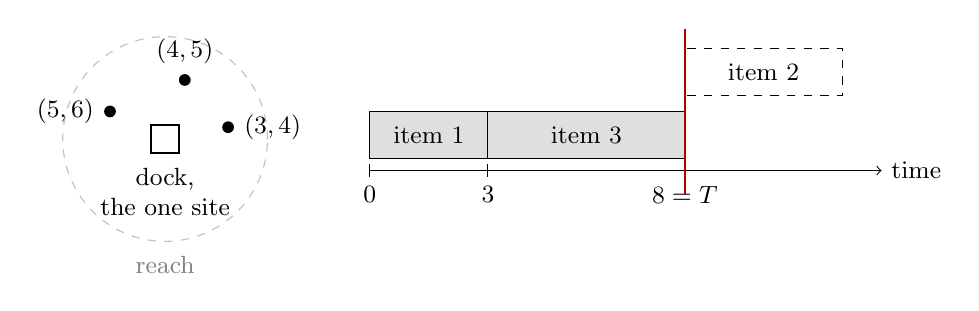
\begin{tikzpicture}[dev/.style={circle, fill=black, inner sep=1.5pt}]
    \draw[gray!50, dashed] (0,0) circle (1.3);
    \node[draw, thick, minimum size=10pt, inner sep=0pt, fill=white] at (0,0) {};
    \node[below=7pt, font=\small, align=center] at (0,0) {dock,\\ the one site};
    \node[dev, label={[font=\small]0:$(3,4)$}] at (0.8,0.15) {};
    \node[dev, label={[font=\small]90:$(4,5)$}] at (0.25,0.75) {};
    \node[dev, label={[font=\small]180:$(5,6)$}] at (-0.7,0.35) {};
    \node[font=\small, gray] at (0,-1.6) {reach};
    \begin{scope}[xshift=2.6cm, yshift=-0.4cm, x=0.5cm]
      \draw[->] (0,0) -- (13,0) node[right, font=\small] {time};
      \foreach \t/\lab in {0/0, 3/3, 8/{$8=T$}}
        \draw (\t,0.08) -- (\t,-0.08) node[below, font=\small] {\lab};
      \draw[fill=gray!25] (0,0.15) rectangle (3,0.75);
      \node[font=\small] at (1.5,0.45) {item 1};
      \draw[fill=gray!25] (3,0.15) rectangle (8,0.75);
      \node[font=\small] at (5.5,0.45) {item 3};
      \draw[dashed] (8,0.95) rectangle (12,1.55);
      \node[font=\small] at (10,1.25) {item 2};
      \draw[red!70!black, thick] (8,-0.3) -- (8,1.8);
    \end{scope}
  \end{tikzpicture}
  \caption{Lemma~\ref{lem:packing}'s instance for items with (size, value)
    $(3,4)$, $(4,5)$, $(5,6)$ and capacity $K=8$. Every device is in reach
    of the dock, the only site (positions drawn apart for clarity), so the
    drone never flies, and a plan is a set of devices sending one after
    another. Items 1 and 3 fill the time limit exactly and are worth $10$;
    item 2 does not fit after them.}
  \label{fig:packing}
\end{figure}

\subsection{The result (step 2.5)}
\label{sec:t1-result}

\begin{theorem}[T1]
\label{thm:t1}
\begin{enumerate}
  \item For every fixed rational $\delta>0$, $\PLAN_\delta$ is NP-complete,
    and NP-complete in the strong sense.
  \item $\PLAN_{\mathrm{ex}}$ is NP-hard in the strong sense. Whether it is
    in NP is open.
  \item Both stay NP-hard with a single radio setting of constant rate, in
    two separate ways: through the route alone, with no data (or equal
    data), no deadlines, every importance $1$ and the sites at the devices;
    and through packing alone, with one site at the dock and no flying.
\end{enumerate}
\end{theorem}

\begin{proof}
Membership in NP for rounded times is Proposition~\ref{prop:np}.
Lemma~\ref{lem:routing} converts an NP-complete problem with no numbers in
it into both versions of \PLAN{}, and its instances have numbers bounded by
a polynomial in $n$. A pseudo-polynomial algorithm for \PLAN{} would
therefore decide \textsc{Hamiltonian Cycle} in grid graphs in polynomial
time, so both versions are NP-hard in the strong sense
\cite[Section~4.2]{GareyJohnson1979}. Part 3 restates the instances of
Lemmas~\ref{lem:routing} and~\ref{lem:packing}. Membership of
$\PLAN_{\mathrm{ex}}$ is discussed in Remark~\ref{rem:exact}.
\end{proof}

\paragraph{What each conversion shows.} The two lemmas make different
claims, and the report keeps them apart.
\begin{itemize}
  \item \emph{The route is hard by itself} (Lemma~\ref{lem:routing}). One
    setting, no sending or the same sending for every device, no
    deadlines, every device equally important, and stops only at the
    devices: what remains is the order of the stops, and that is already
    hard. It is hard in the strong sense, so no dynamic program over time,
    the kind that solves knapsack, can solve \PLAN{} in general unless
    $\mathrm{P}=\mathrm{NP}$. By Remark~\ref{rem:code-model} this covers the
    planner's own kind of instance.
  \item \emph{Packing is hard by itself} (Lemma~\ref{lem:packing}). No
    flying at all and a single stop: what remains is which devices to
    serve within the time, and that is knapsack. This hardness is only in
    the weak sense, and it needs devices with different send times.
    Proposition~\ref{prop:one-stop-equal} shows that the planner's
    instances, where every device sends the same data and a setting has
    at most $15$ rates, do not have it.
  \item \emph{Choosing the setting adds nothing.} A plan uses one setting,
    and whether it is valid depends on that setting alone. So the best plan
    over $|B|$ settings is the best of $|B|$ one-setting problems, solved
    separately: for FeRRy, three. The planner does the same, one search
    per setting.
\end{itemize}

\subsection{Simpler versions (step 2.6)}
\label{sec:t1-simpler}

Table~\ref{tab:simpler} settles the simpler versions. A running time is
\emph{pseudo-polynomial} when it is polynomial in $n$, $|P|$, $|B|$ and the
time limit $T$, with send times written as integers. (If $T=\infty$, read
$T$ as the total send time of all devices.) In
Propositions~\ref{prop:one-stop} to~\ref{prop:one-site}, the drone flies
from the dock to a site $p$ and back, so the flying is a constant: write
$\alpha_p=\tau(o,p)$ and $\beta_p=\tau(p,o)+u$. Device $j$, served at $p$,
must finish by its \emph{latest finish} $L_j=\min(D_j,\,T-\beta_p)$, and has
\emph{room} $E_j=L_j-\alpha_p$ for sending, its own included.

\begin{table}[t]
  \centering
  \small
  \begin{tabular}{@{}p{0.36\linewidth}p{0.27\linewidth}p{0.29\linewidth}@{}}
    \toprule
    Version & Complexity & How \\
    \midrule
    One setting & strongly NP-hard & Lemma~\ref{lem:routing} \\
    Several settings & no harder than one & best of $|B|$ one-setting runs \\
    Exact or rounded travel & both strongly NP-hard & Lemma~\ref{lem:routing} \\
    No data or equal data, no deadlines, importance $1$ & strongly NP-hard & Lemma~\ref{lem:routing}, Remark~\ref{rem:code-model} \\
    The planner's plans only (own group's stop, no repeats) & strongly NP-hard & Remark~\ref{rem:code-model} \\
    \midrule
    At most one stop & NP-hard (weakly); pseudo-polynomial & Lemma~\ref{lem:packing}; Prop.~\ref{prop:one-stop} \\
    At most one stop, equal send times & polynomial & Prop.~\ref{prop:one-stop-equal}(a) \\
    At most one stop, equal data, $K$ rate steps & polynomial for fixed $K$; NP-hard if $K$ is unbounded & Prop.~\ref{prop:one-stop-equal}(b), (c) \\
    One site, repeat visits, deadlines & NP-hard (weakly); pseudo-polynomial & Prop.~\ref{prop:one-site}(a) \\
    One site, equal send times, deadlines & polynomial, greedy & Prop.~\ref{prop:one-site}(b) \\
    At most $k$ stops, $k$ fixed & NP-hard (weakly) for $k\ge1$; pseudo-polynomial & Prop.~\ref{prop:k-stops} \\
    At most $k$ stops, equal send times & polynomial for fixed $k$ & Prop.~\ref{prop:k-stops} \\
    \bottomrule
  \end{tabular}
  \caption{Simpler versions of \PLAN{}. ``Equal send times'' means every
    device sends for the same time wherever it is served: equal data and
    one rate per setting.}
  \label{tab:simpler}
\end{table}

\begin{proposition}[At most one stop]
\label{prop:one-stop}
\PLAN{} restricted to plans with at most one stop is NP-hard. With integer
send times it is solved in $O(|B|\,|P|\,n\,T)$ time.
\end{proposition}

\begin{proof}
In Lemma~\ref{lem:packing}'s instances, merging all stops of a valid plan
into one stop at the dock keeps it valid (all legs cost $0$ and there are no
deadlines) and keeps its value, so the restricted problem has the same
answer. For the algorithm, fix a setting $b$ and a site $p$, and let $R$ be
the devices in reach of $p$, with send times $\sigma_j$. A single stop
serving $S\subseteq R$ finishes at $\alpha_p+\sigma(S)$, where
$\sigma(S)=\sum_{j\in S}\sigma_j$, so it is valid exactly when
$\sigma(S)\le\min_{j\in S}E_j$. Order $R$ by decreasing room,
$E_{(1)}\ge E_{(2)}\ge\cdots$. In a valid $S$, the device that comes last in
this order has the least room. So the best stop whose last device is $(t)$
consists of $(t)$ and the most valuable subset of $(1),\dots,(t-1)$ with
total send time at most $E_{(t)}-\sigma_{(t)}$. A knapsack table over
$(1),\dots,(t-1)$, extended one device at a time, answers this for every
$t$ in $O(|R|\,T)$ time, since no valid stop sends for longer than $T$. The
best over all $b$, $p$ and $t$, or the empty plan, is optimal.
\end{proof}

\begin{proposition}[At most one stop, equal data]
\label{prop:one-stop-equal}
Let every device have the same data size, and restrict to plans with at
most one stop.
\begin{enumerate}
  \item[(a)] If every setting has one rate, the problem is solved in
    $O(|B|\,|P|\,n^2)$ time. Without deadlines, the best stop serves the
    most important devices in reach, as many as fit.
  \item[(b)] If every setting has at most $K$ rate steps, it is solved in
    $O(|B|\,|P|\,K\,n^{K})$ time: polynomial for fixed $K$, such as the
    planner's at most $15$ rates.
  \item[(c)] If the number of rate steps is part of the input, it is
    NP-hard, even with one site at the dock.
\end{enumerate}
\end{proposition}

\begin{proof}
Fix $b$ and $p$, and order $R$ by decreasing room as in
Proposition~\ref{prop:one-stop}. (a) Every send time is the same $\sigma$,
so the best stop whose last device is $(t)$ serves $(t)$ and the
$\lfloor E_{(t)}/\sigma\rfloor-1$ most important of $(1),\dots,(t-1)$ (none
if $E_{(t)}<\sigma$). Keeping $(1),\dots,(t-1)$ sorted by importance with
prefix sums gives each $t$ in $O(n)$ time. Without deadlines every room is
$T-\beta_p-\alpha_p$, so the best stop takes the
$\lfloor(T-\beta_p-\alpha_p)/\sigma\rfloor$ most important devices.
(b) Send times now take at most $K$ values, one per step, so the devices
fall into $K$ classes of equal send time. Taking $k$ devices from a class,
the $k$ most important are best. For each $t$, try every count for $K-1$
of the classes, at most $n^{K-1}$ choices, and take from the last class as
many as still fit. With prefix sums per class this is $O(K)$ per choice.
(c) Convert \textsc{Knapsack} as in Lemma~\ref{lem:packing}, but give every
device data size $1$. Let $a^{(1)}<\dots<a^{(q)}$ be the distinct item
sizes. The setting has reach $1$ and steps $d_i=i/q$ with rates
$\rho_i=1/a^{(i)}$, which never increase. An item of size $a^{(i)}$ stands
$i/q$ from the dock, so it sends at $\rho_i$ for $a^{(i)}$ seconds. The rest
of Lemma~\ref{lem:packing}'s proof is unchanged.
\end{proof}

Part (c) sharpens the lead recorded in Phase~1. The knapsack conversion
needs devices with \emph{different send times}. Different data sizes give
them, and so do many rate steps with equal data. The planner's instances
have neither, since they have equal data and at most $15$ rates, so their
one-stop case is polynomial by part (b). Their hardness comes from the
route (Remark~\ref{rem:code-model}).

\begin{proposition}[One site, repeat visits]
\label{prop:one-site}
Let $P=\{p\}$, so the drone may stop at $p$ several times but nowhere else.
\begin{enumerate}
  \item[(a)] The problem is NP-hard. With integer send times it is solved
    in $O(|B|\,n\,T)$ time.
  \item[(b)] If every send time is the same, the greedy rule is optimal:
    consider the devices by decreasing importance, and keep each one if the
    kept devices can still all be served on time. It runs in $O(|B|\,n^2)$
    time.
\end{enumerate}
\end{proposition}

\begin{proof}
Splitting a stop into one-device stops, kept in order at the same site,
keeps a plan valid: each device is then checked at its own finish, which is
no later than the old stop's finish, and the last finish is unchanged. So
every stop may serve one device. A plan is then an ordered set $S$ of
devices sending one after another from time $\alpha_p$. Device $j$ finishes
at $\alpha_p$ plus the send times up to and including its own, and must
finish by $L_j$. (The time limit binds the last finish, which is the
latest, so putting it in every $L_j$ changes nothing.) If some order of $S$
meets every $L_j$, the order by increasing $L_j$ does. Swapping two
neighbours that are out of order finishes the earlier-due one sooner than
before. The later-due one now finishes at the pair's old finish, which met
the earlier due time and so meets its own. Repeated swaps sort the
order. This is single-machine scheduling to maximize the importance of the
devices on time. (a) Lemma~\ref{lem:packing}'s instances have one site, so
the problem is NP-hard. The dynamic program of Lawler and Moore
\cite{LawlerMoore1969} goes through the devices by increasing $L_j$ and
keeps the best value for each total send time, in $O(n\,T)$ time per
setting. (b) With every send time $\sigma$, device $j$ can be the $t$-th
served exactly when $t\le\ell_j=\lfloor E_j/\sigma\rfloor$. A set $S$ is
valid exactly when, for every $t$, at most $t$ of its devices have
$\ell_j\le t$. These sets are the independent sets of a matroid
\cite[Section~16.5]{CLRS2009}, so the greedy rule is optimal. Each test of
a kept set takes $O(n)$ time.
\end{proof}

With equal data and $K$ rate steps the send times at one site take at most
$K$ values. Running the same dynamic program with the number of devices
taken from each class as its state gives $O(|B|\,n^{K+1})$ time:
polynomial for fixed $K$.

\begin{proposition}[At most $k$ stops]
\label{prop:k-stops}
Fix $k\ge1$ and restrict to plans with at most $k$ stops. The problem is
NP-hard. With integer send times it is solved in
$O(|B|\,|P|^k\,n^{k+1}\,k\,T^{k})$ time, and without deadlines in
$O(|B|\,|P|^k\,n\,T)$. If every send time is the same, it is solved in
polynomial time.
\end{proposition}

\begin{proof}
NP-hardness is Proposition~\ref{prop:one-stop}'s, since a plan with at most
one stop has at most $k$. For the algorithms, try every setting and every
list of at most $k$ sites, at most $|B|\,|P|^k$ choices. That fixes the
route: the flying time $\Lambda_l$ to stop $l$ and the time $\beta$ home
with the upload. What is left is to give each served device a stop in reach
of it. By~\eqref{eq:finish}, if $y_l$ is the send time at stop $l$, then
$f_l=\Lambda_l+y_1+\dots+y_l$.
A stop left empty is dropped, which by the triangle inequality makes no
later time later.
\emph{Without deadlines} only the total matters, $\Lambda_m+\sum_l
y_l+\beta\le T$. So each device is best served at the stop where it sends
fastest, and one knapsack over these send times, of capacity
$T-\Lambda_m-\beta$, finishes the job.
\emph{With deadlines}, also guess for each stop the device with the
earliest deadline it serves, at most $n^k$ guesses, and place it there. A
stop may then serve only devices with a deadline no earlier than its
guessed one, $D^*_l$, and the conditions become
$\Lambda_l+y_1+\dots+y_l\le D^*_l$ for each $l$, plus the time limit. A
dynamic program over the other devices, whose state is $(y_1,\dots,y_k)$
with each $y_l\le T$, decides each device's stop in $O(k\,T^k)$ time per
device.
\emph{With equal send times} $\sigma$, guess instead how many devices each
stop serves, at most $(n+1)^k$ guesses. This fixes every finish $f_l$.
Device $j$ may go to stop $l$ when $p_l$ is in reach and $f_l\le D_j$. The
best choice is a maximum-importance assignment of devices to stops within
the guessed counts, a bipartite matching problem solved in polynomial time.
Serving fewer than the guessed count only makes every later stop earlier,
so every assignment found is valid.
\end{proof}

\paragraph{What T1 says about FeRRy's planner.} The planner's problem, in
the simplified form, is strongly NP-hard, and so is the smaller set of plans
the planner searches (Remark~\ref{rem:code-model}). The hardness is in the
route. With equal data and at most $15$ rates, the planner's one-stop and
one-site cases are polynomial (Propositions~\ref{prop:one-stop-equal}(b)
and~\ref{prop:one-site}). Choosing among the three settings multiplies the
work by three and adds no hardness. So the planner's shortcuts that matter
for Q2 are the ones that order and choose stops, its 2-opt start and local
search. T2 and T3 measure and bound what they lose.
